\section{An Introduction to Mobile Edge Computing}  \label{intro}


Toward 5G networks and the fourth industries, Telco companies and service providers are facing with tremedous oppotunities and challenges. One of them is to support innovative mobile applications, which require new generations of smart devices (e.g., AR/VR and smartphone) that are quickly released. Such a phenomenon results in an explosion of data. The fact is that 63\% of the world population currently acquires a mobile subscription, meanwhile, it was just 20\% in the previous decade. In addition, new use cases such as Internet of Things (IoT) and Machine-Type-Communications (MTC) introduce a huge number of connections, which shows promising business opportunities for mobile operators.

Considering the potential benefits from processing the huge amount of data, there is a need to design a cloud architecture. However, to ease the service management, the current cloud design follows a conventional centralized way that introduces major limiations, which could hardly apply for the emerging use cases. One of the main weaknesses is that the centralized cloud architecture introduces significant execution delay. In addition, such a design also shows the inflexibility, especially for services which require high availability and high mobility. 

Mobile Edge Computing (MEC) was presented as a new technology, which fills the gaps of the centralized cloud design, whereby the cloud services are moved to a proximity of the end users. An example shown  in Fig.~\ref{fig:mec-arch} shows that the services can be located at the edge of the mobile networks (i.e., base stations). MEC is designed to serve various use cases such as Augmented Reality/Virtual Reality applications, autonomous vehicles, smart city, and health care.


\begin{figure}[H]
  \begin{center}
   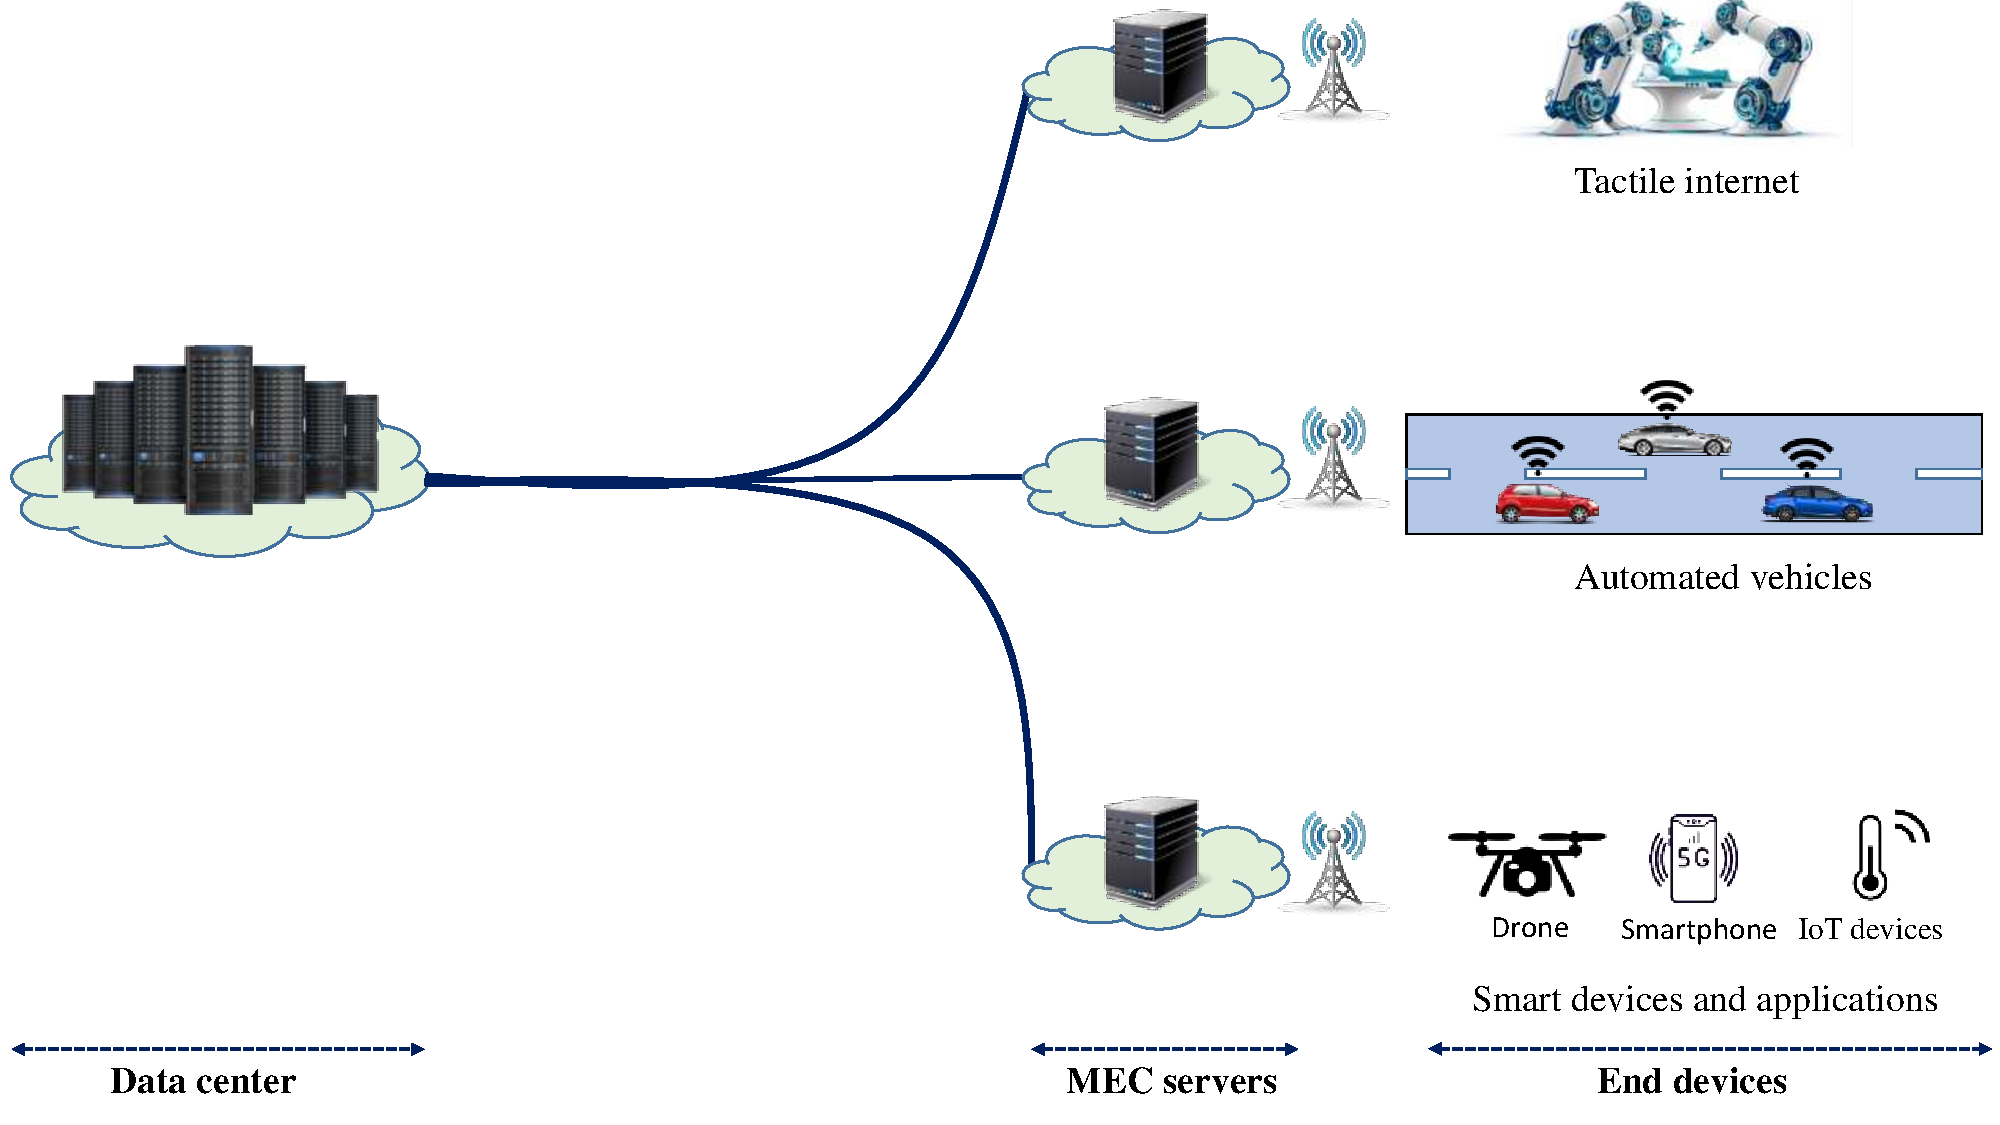
\includegraphics[width=13cm]{./figures/mec-arch.pdf}
   \caption{An example of MEC architecture}
   \label{fig:mec-arch}
   \end{center}
\end{figure}
